\documentclass[a4paper,14pt]{article}

\usepackage[12pt]{extsizes}
\usepackage{cmap}                   % поиск в PDF
\usepackage{mathtext}               % русские буквы в формулах
\usepackage[T2A]{fontenc}           % кодировка
\usepackage[utf8]{inputenc}         % кодировка исходного текста
\usepackage[english,russian]{babel} % локализация и переносы
\usepackage{graphicx}
\usepackage{geometry}
\usepackage{amsmath}
\usepackage{amssymb}
\usepackage[table]{xcolor}
\usepackage{indentfirst}
\setlength\extrarowheight{2pt}

\geometry{verbose, a4paper, tmargin=2cm, bmargin=2cm, lmargin=3cm, rmargin=1.5cm}
\author{Высоцкий Максим}
\title{Отчёт по лабораторной работе 1.1}
\date{2025}

\begin{document}
    \begin{titlepage}
        \begin{center}
            Министерство науки и высшего образования Российской Федерации \\
            НОВОСИБИРСКИЙ НАЦИОНАЛЬНЫЙ ИССЛЕДОВАТЕЛЬСКИЙ \\
            ГОСУДАРСТВЕННЫЙ УНИВЕРСИТЕТ (НГУ)
        \end{center}
        
        \begin{center}
            Физический факультет
        \end{center}
        
        \begin{center}
            Кафедра общей физики
        \end{center}
        
        \vspace{7cm}
        \begin{center}
            \textbf{Лабораторная работа №1.1} \\
            \textbf{Броуновское движение частиц в жидкости}
        \end{center}
        
        \vspace{2cm}
        \begin{flushright}
            Руководитель: \\
            Ассистент Художитков В. Э. \\
            Старший преподаватель Кравцова А. Ю. \\
            \vspace{1cm}
            Работу выполнил: \\
            Высоцкий М. Ю. \\
            гр. 24301
        \end{flushright}
        
        \vspace{3cm}
        \begin{center}
            Новосибирск, 2025
        \end{center}
    \end{titlepage}
\thispagestyle{empty}
\section*{Аннотация}
В данной работе исследовалось броуновское движение частиц в жидкости с использованием микроскопа ОМ-П с веб-камерой. Были определены: коэффициент перевода пикселей в микрометры, диаметр броуновской частицы и коэффициент диффузии. Экспериментально проверены законы Эйнштейна-Смолуховского для броуновского движения. Полученные значения коэффициента диффузии составили $D \approx 171 \frac{\text{мкм}^2}{\text{с}}$, что согласуется с теоретическими предсказаниями. Работа демонстрирует статистическую природу теплового движения микрочастиц.

\clearpage

\tableofcontents
\thispagestyle{empty}
\clearpage

\section{Введение}
Броуновское движение - это беспорядочное тепловое движение малых частиц, взвешенных в жидкости или газе, впервые наблюдаемое Р. Броуном в 1827 году. Теоретическое объяснение этого явления было дано А. Эйнштейном и М. Смолуховским в 1905-1906 годах, что стало важным подтверждением молекулярно-кинетической теории.

Актуальность исследования броуновского движения сохраняется и в настоящее время, особенно в связи с развитием нанотехнологий, где понимание поведения частиц на микро- и наноуровне имеет принципиальное значение.

Целью данной работы является экспериментальное изучение законов броуновского движения, определение коэффициента диффузии и проверка соотношений Эйнштейна-Смолуховского. В работе использовались современные методы визуализации и компьютерной обработки данных, что позволяет получить точные количественные результаты.

\section{Теоретическая часть}
Броуновское движение возникает вследствие хаотического теплового движения молекул среды, вызывающего флуктуации импульса, передаваемого взвешенным частицам. В жидкости эти флуктуации обусловлены перестройкой межмолекулярных связей.

\begin{figure}[h]
    \centering
    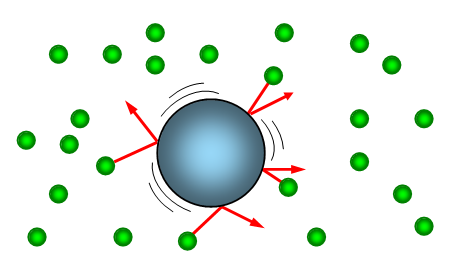
\includegraphics[width=0.6\textwidth]{brown.png}
    \caption{Схематическое изображение броуновского движения частицы}
    \label{fig:brown}
\end{figure}

Движение броуновских частиц принципиально отличается от движения макроскопических тел:
\begin{itemize}
    \item Траектория частицы не имеет производных (в каждой точке "излом")
    \item Классические понятия скорости и ускорения неприменимы
    \item Движение описывается вероятностными, а не детерминированными законами
\end{itemize}

Согласно первому закону Эйнштейна-Смолуховского, средний квадрат смещения частицы пропорционален времени:
\begin{equation}
    \langle \Delta x^2 \rangle = 2Dt
    \label{eq:first_law}
\end{equation}

Коэффициент диффузии $D$ определяется вторым законом:
\begin{equation}
    D = \frac{kT}{6\pi\eta a}
    \label{eq:second_law}
\end{equation}
где $k$ - постоянная Больцмана, $T$ - температура, $\eta$ - вязкость среды, $a$ - радиус частицы.

\section{Экспериментальная часть}
\subsection{Описание установки}
Экспериментальная установка состояла из: микроскопа "Биолам" с объективом ×40, подключенной веб-камеры c разрешениеем 1280×1024 пикселей, компьютера с программой "Brownian" для обработки данных, микрокюветы с исследуемой жидкостью, эталонного объект-микрометра для калибровки.


\begin{figure}[h]
    \centering
    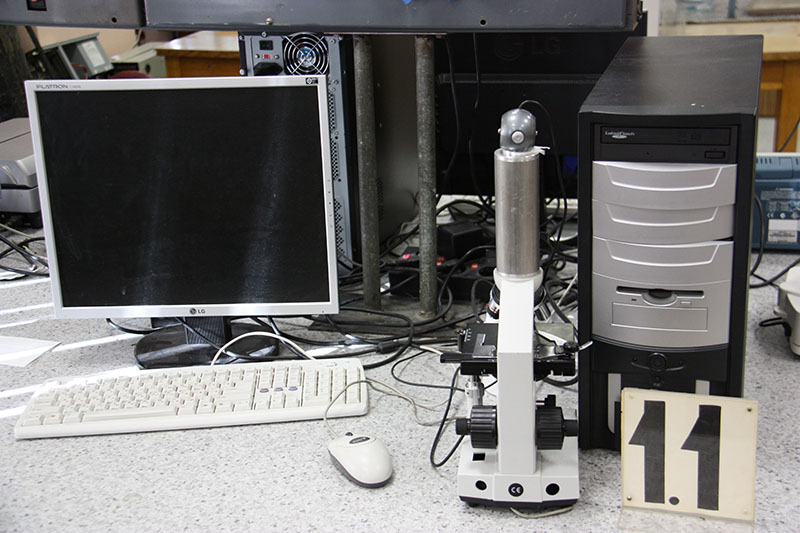
\includegraphics[width=0.7\textwidth]{setup.jpg}
    \caption{Схема экспериментальной установки}
    \label{fig:setup}
\end{figure}

\subsection{Методика измерений}
В данной работе требуется подготовить препарат (микрокювету) с жидкостью. Микроскоп устанавливается на расстоянии около 2 мм. от препарата, ставится объектив ×40. Далее делается серия из 200 фотографий с интервалом в 1 секунду. Затем вместо препарата ставится шкала микрометра. Обработка производится при помощи вспомогательного ПО, где можно получить координаты частицы. Также при помощи данного ПО можно посчитать перевод пикселей в мкм.

\section{Результаты измерений}
Была получена траектория броуновской частицы, состоящая из 200 положений с интервалом в 1 секунду. После обработки были получены координаты частицы в каждый момент времени (200 шт.), траектория частицы изображена на рисунке \ref{fig:trajectory}. Для перевода координат из пикселей в микрометры использовалось калибровочное изображение, для его мы использовали микрометр. Данные для этой части эксперимента приведены в таблице 1. Среднее смещение составило $\overline{\Delta x} \approx 98,88$ мкм. Посчитан коэффициент пересчета: 10 пикселей = 1 мкм ($\aleph = 1/10$).

\begin{figure}[h]
    \centering
    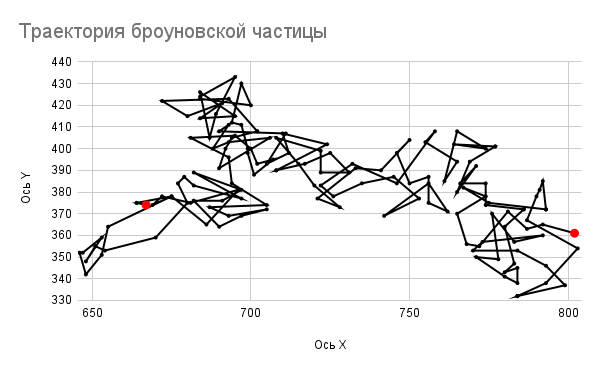
\includegraphics[width=0.8\textwidth]{trajectory.png}
    \caption{Траектория броуновской частицы. Красным отмечены начальная и конечная точки.}
    \label{fig:trajectory}
\end{figure}


\clearpage
\begin{table}[h]
    \centering
    \caption{Координаты частицы и смещения}
    \begin{tabular}{|l|l|l|}
    \hline
        $x$ (пикс) & $y$ (пикс) & $\Delta x$ (пикс) \\ \hline
        24  & 148 &  \\ \hline
        121 & 148 & 97 \\ \hline
        216 & 152 & 95 \\ \hline
        321 & 154 & 105 \\ \hline
        415 & 156 & 94 \\ \hline
        516 & 156 & 101 \\ \hline
        616 & 156 & 100 \\ \hline
        713 & 159 & 97 \\ \hline
        815 & 159 & 102 \\ \hline
    \end{tabular}
    \label{tab:coordinates}
\end{table}

По полученным данным из 200 координат, построены зависимости $\langle \Delta x^2 \rangle$, $\langle \Delta y^2 \rangle$ и их среднего от времени:

\begin{figure}[h]
    \centering
    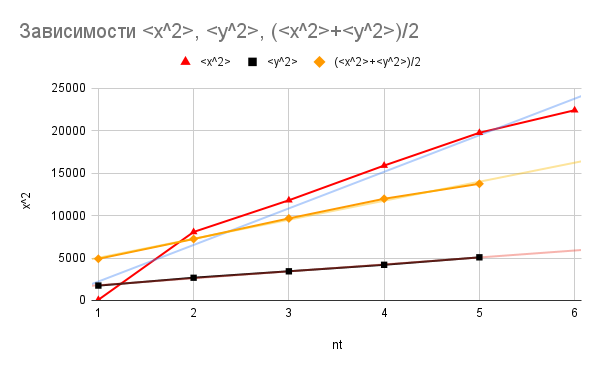
\includegraphics[width=0.9\textwidth]{graph.png}
    \caption{Зависимость L^2 $\left(\langle \Delta x^2 \rangle, \langle \Delta y^2 \rangle, \frac{\langle \Delta x^2 \rangle + \langle \Delta y^2 \rangle}{2}\right)$ от $t=n\tau$}
    \label{fig:graph}
\end{figure}

По наклону графиков определен коэффициент диффузии:
$$ D \approx 171 \frac{\text{мкм}^2}{\text{с}} $$

Диаметр наблюдаемой частицы составил $d \approx 1,8$ мкм.

Полученные значения $\langle \Delta x^2 \rangle$ и коэффициента диффузии $D$ оказались достаточно большими, что объясняется значительной свободой движения частицы в исследуемой среде. Это согласуется с визуальными наблюдениями - частица преодолевала большие расстояния за время эксперимента.

Погрешности измерений связаны с:
\begin{itemize}
    \item Ограниченной точностью определения координат с помощью мыши
    \item Конечным временем наблюдения
    \item Возможными микротечениями в жидкости
\end{itemize}

\section{Выводы}
Экспериментально подтверждена линейная зависимость среднего квадрата смещения броуновской частицы от времени (первый закон Эйнштейна-Смолуховского), был определен коэффициент перевода пикселей в микрометры: $\aleph = 1/10$ (10 пикселей = 1 мкм), также измерен диаметр броуновской частицы: $d = 1,8$ мкм. Затем, рассчитан коэффициент диффузии: $D = 171 \frac{\text{мкм}^2}{\text{с}}$. Таким образом, была продемонстрирована статистическая природа броуновского движения.

В ходе работы были успешно выполнены все поставленные задачи. Полученные результаты хорошо согласуются с теоретическими предсказаниями. Работа позволила на практике познакомиться с особенностями броуновского движения и методами его исследования.

\begin{thebibliography}{9}
\bibitem{manual} 
Смирных Л.Н., Дорошкин А.А. Броуновское движение частиц в жидкости: Методические указания к лабораторной работе / Новосиб. гос. ун-т. - Новосибирск, 2010. - 16 с.

\bibitem{sivukhin} 
Сивухин Д.В. Общий курс физики. Т. II. Термодинамика и молекулярная физика. - 5-е изд., стер. - М.: Физматлит, 2005. - 544 с.
\end{thebibliography}

\end{document}